%\section{First and Second}
\section{Result Prediction based on First and Second Segment (Bat First)} 
As we have divided our total model into three segment and we actually consider first two segment for predicting the match outcome as we wanted to find out the final match result when match is in progress. We have taken total 91 match for making our model using multiple linear regression and we have merged all the attributes from those matches based on different segment. After analyzing those two segment our model has given 75\% accuracy. So, we can predict any match outcome when the match is in progress based on our model. As we did not take any attributes from the team who will bat second and considering the attribute which we got from first segment, our predicted model is quite good.

\begin{figure}[htbp]
\centering
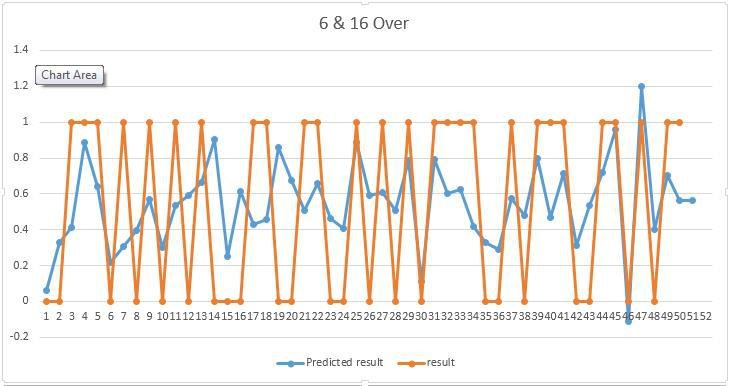
\includegraphics[scale=0.5]{images/fig-17.jpg}
\caption{First and Second Segment Prediction (Bat First)}
\label{fig:x First and Second Segment Prediction (Bat First)}
\end{figure}

From the figure above we can see the graph view of our model, here 0 means lost and 1 means win. So, if the predictive final value is less than 0.5 then the result would be consider as lose and if the predictive value is greater than 0.5 then it would be consider as win.

\textbf{Coefficient:} These are the coefficients values for all the attributes from Win prediction based on bat first.

\begin{table}[htbp]
\centering
\begin{tabular}{l | l}
Attributes & Coefficients\\
\hline
Intercept & 0.092219\\
Venue & 0.242112\\
M6ORN & 0.039573\\
M6OW & -0.12872\\
M16ORN & 0.05121\\
M16OW & -0.07214
\end{tabular}
\caption{First and Second Coefficient (Bat First)}
\label{tab:First and Second Coefficient (Bat First)}
\end{table}

\textbf{P-values:} These are the p values for all the at-tributes from Win prediction based on bat first.

\begin{table}[htbp]
\centering
\begin{tabular}{|l | r|}
\hline
Attributes & P-value\\
\hline
Intercept & 0.87596\\
\hline
Venue & 0.088577\\
\hline
M6ORN & 0.323375\\
\hline
M6OW & 0.084286\\
\hline
M16ORN & 0.246463\\
\hline
M16OW & 0.254117\\
\hline
\end{tabular}
\caption{First and Second Segment P-value (Bat First)}
\label{tab:First and Second Segment P-value (Bat First)}
\end{table}

\section{Result Prediction based on First and Second Segment (Bat Second)} 
While calculating for 2nd innings segments we get the run rate value from team batting first. Which makes a better impact on a prediction model and that time our model has given 85.5\% accuracy which is really good.

\begin{figure}[htbp]
\centering
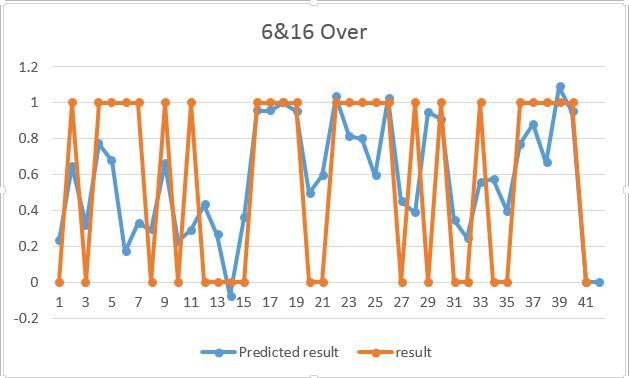
\includegraphics[scale=0.5]{images/fig-18.jpg}
\caption{First and Second Segment Run Prediction (Bat Second)}
\label{fig:x Frist and Second Segment Run Prediction (Bat Second)}
\end{figure}

\textbf{Coefficient:} These are the coefficients values for all the attributes from Win prediction based on bat second.
\vspace{3cm}

\begin{table}[htbp]
\centering
\begin{tabular}{|l | l|}
\hline
Attributes & Coefficients\\
\hline
Intercept & 2.282567\\
Venue & -0.04063\\
M6ORN & -0.02869\\
M6OW & -0.22694\\
M16ORN & -0.12705\\
M16OW & -0.10903\\
O6ORN & 0.008056\\
060W & 0.066748\\
O16ORN & 0.028731\\
O16OW & -0.0978\\
\hline
\end{tabular}
\caption{First and Second Segment Coefficient (Bat Second)}
\label{tab:First and Second Segment Coefficient (Bat Second)}
\end{table}

\textbf{P-values:} These are the p values for all the at-tributes from Win prediction based on bat second.

\setlength{\arrayrulewidth}{0.5mm}
\setlength{\tabcolsep}{12pt}
\renewcommand{\arraystretch}{1.5}

\begin{table}[ht]
\centering
\begin{tabular}{|l | l|}
\hline
\multicolumn{2}{| c |}{First and Second Segment P-value (Bat Second)} \\
\hline
Attributes & Coefficients\\
\hline
Intercept & 0.007165\\
Venue & 0.811504\\
M6ORN & 0.482433\\
M6OW & 0.019258\\
M16ORN & 0.112474\\
M16OW & 0.090761\\
O6ORN & 0.878555\\
060W & 0.429492\\
O16ORN & 0.633494\\
O16OW & 0.179298\\
\hline
\end{tabular}
\caption{First and Second Segment P-value (Bat Second)}
\label{tab:First and Second Segment P-value (Bat Second)}
\end{table}
